\chapter{Implementare}
\pagestyle{headings}

\section{Considera'tii generale}

Proiectul este dezvoltat pe platforma Windows 7, utiliz{\ia}nd editorul integrat Visual Studio 2012. Acesta dispune de un subset al standardului C++ pe care 'il putem folosi 'in dezvoltarea proiectului. Pentru a asigura portabilitatea proiectului, vom utiliza utilitarul \emph{Premake} pentru a descrie fisierele sursa utilizate de proiect 'si dependin'tele acestora. Utilitarul Premake va genera pe baza unui fi'sier descriptiv un proiect Visual Studio. 

\medskip

Proiectul este 'imp'ar'tit in urm'atoarele foldere: \emph{binaries} este folderul unde se va genera binarul executabil al proiectului, \emph{build} este folderul unde se afl'a fi'sierele necesare compil'arii proiectului, \emph{doc} este folderul unde se afl'a documenta'tia proiectului in format Latex, \emph{include} con'tine fi'sierele header ale bibliotecii, \emph{src} con'tine fi'sierele surs'a ale bibliotecii, \emph{demo} con'tine fi'sierele surs'a ale aplica'tiei demonstrative iar \emph{tests} con'tine fi'sierele surs'a ale proiectului de testare a bibliotecii.

\medskip

Proiectul este 'imp'ar'tit in 3 sub-proiecte: biblioteca wxStyle, aplica'tia demonstrativ'a 'si proiectul de testare a bibliotecii. Biblioteca poate fi compilat'a static sau dinamic. Aplica'tia demonstrativ'a 'si proiectul de testare se compileaz'a in fi'siere binare executabile. Biblioteca va utiliza namespace-ul \emph{wxstyle} pentru toate obiectele pe care le expune.

\subsection{Pointer to Implementation (PIMPL)}

Pentru a maximiza encapsularea componentelor din interiorul bibliotecii wxStyle 'si pentru a facilita un proces de dezvoltare mai rapid, proiectul folose'ste paradgima PIMPL, adic'a \emph{Pointer to Implementation}. Aceasta  presupune ca membrii (implementarea) unei clase s'a fie encapsula'ti 'intr-un obiect privat unit'a'tii de translatare, iar clasa respectiv'a s'a con'tina doar un pointer c'atre obiectul privat. 'In acest fel, schimb'arile in implementarea unei clase nu afecteaz'a interfa't'a acesteia vizibila 'in fi'sierele header, 'si nu modific'a dimensiunea sau reprezentarea binar'a a acesteia. Din acest motiv, timpii de compilare scad exponen'tial.

\subsection{Managementul resurselor (RAII)}

Limbajul de programare C++ garanteaz'a executarea metodelor de tip destructor 'in momentul 'in care obiectele i'si termin'a via'ta. Din acest motiv, destructorii sunt locul potrivit eliberarea resurselor precum memoria. Obiectele care procur'a resurse 'in cadrul constructorului 'si elibereaz'a aceste resurse 'in cadrul destructorului se numesc \emph{Resource Handlers}. Resursa principal'a administrat'a 'in acest mod este memoria, iar obiectele care administreaz'a memoria se numesc \emph{Smart Pointers}. Biblioteca wxStyle utilizeaz'a smart pointers pentru administrarea memoriei.

% ==============================================================================
%   Obiecte de interfata
% ==============================================================================

\section{Obiecte de Interfa't'a}

Datorit'a implement'arii bibliotecii wxWidgets, mai precis decizia de a folosi obiecte de interfa't'a native 'in spatele unor interfe'te abstractizate, modul de prezentare al acestor obiecte este nativ platformei pe care se executa aplica'tia. De'si o tr'as'atur'a avantajoas'a a bibliotecii, acest lucru 'impedic'a specializarea prezent'arii obiectelor. Singura solu'tie este reimplementarea obiectelor de interfa't'a cu suport pentru stilizare incorporat. Obiectele implementate de biblioteca wxStyle sunt prezentate in tabelul \ref{comp_tech_int}

\begin{center}
\begin{figure}[H]
    \centering
    \begin{tabular}{ |p{2.5cm}|p{3cm}|p{9.1cm}| }
        \hline
        \textbf{wxWidgets} & \textbf{wxStyle} & \textbf{Descriere} \\
        \hline
        wxWindow            & StyledWindow      & R'ad'acina ierarhiei  \\
        wxFrame             & StyledFrame       & Reprezint'a o fereastr'a (window)\\
        wxStaticText        & StyledLabel       & Reprezint'a informa'tie sub forma de text 'si icoan'a \\
        wxButton            & StyledButton      & Permite ac'tionarea unui buton prin ap'asare \\
        wxCheckBox          & StyledCheckBox    & Permite reprezentarea unei valori logice \\
        wxTextCtrl          & StyledTextBox     & Permite editarea de text \\
        \hline
    \end{tabular}
    \caption{Asociere 'intre obiectele de interfa't'a implementate in wxStyle 'si cele implementate in wxWidgets}
    \label{comp_tech_int}
\end{figure}
\end{center}



% ==============================================================================
%   Styled Window
% ==============================================================================

\subsection{StyledWindow}

Clasa StyledWindow st'a la r'ad'acina ierarhiei de clase ce reprezint'a obiectele de interfa't'a din wxStyle. Aceast'a clas'a are dou'a roluri fundamentale:

StyledWindow cuprinde toate propriet'a'tile 'si aspectele comune ale obiectelor de interfa't'a stilizabile, 
StyledWindow realizeaz'a o legatur'a dintre ierarhia de obiecte stilizabile implementate in cadrul libr'ariei wxStyle 'si ierarhia obiectelor de interfa't'a implementate in wxWidgets. 

\medskip

Pentru a 'indeplini rolul 2, clasa p'arinte a clasei StyledWindow este wxWindow. wxWindow este clasa de baz'a pentru toate obiectele de interfa't'a din wxWidgets. Prin aceast'a leg'atur'a de mo'stenire, toate obiectele ce implementeaz'a clasa StyledWindow pot fi folosite oriunde poate fi folosit un obiect de interfa'ta implementat 'in wxWidgets. Mai mult, prin aceast'a legatur'a clasa StyledWindow devine EventHandler 'si este eligibil'a s'a primeasc'a evenimente generate de sistemul de operare 'si administrate de wxWidgets.\ref{ch5_class_system_architecture} 

\begin{center}
\begin{figure}[h]
    \centering
    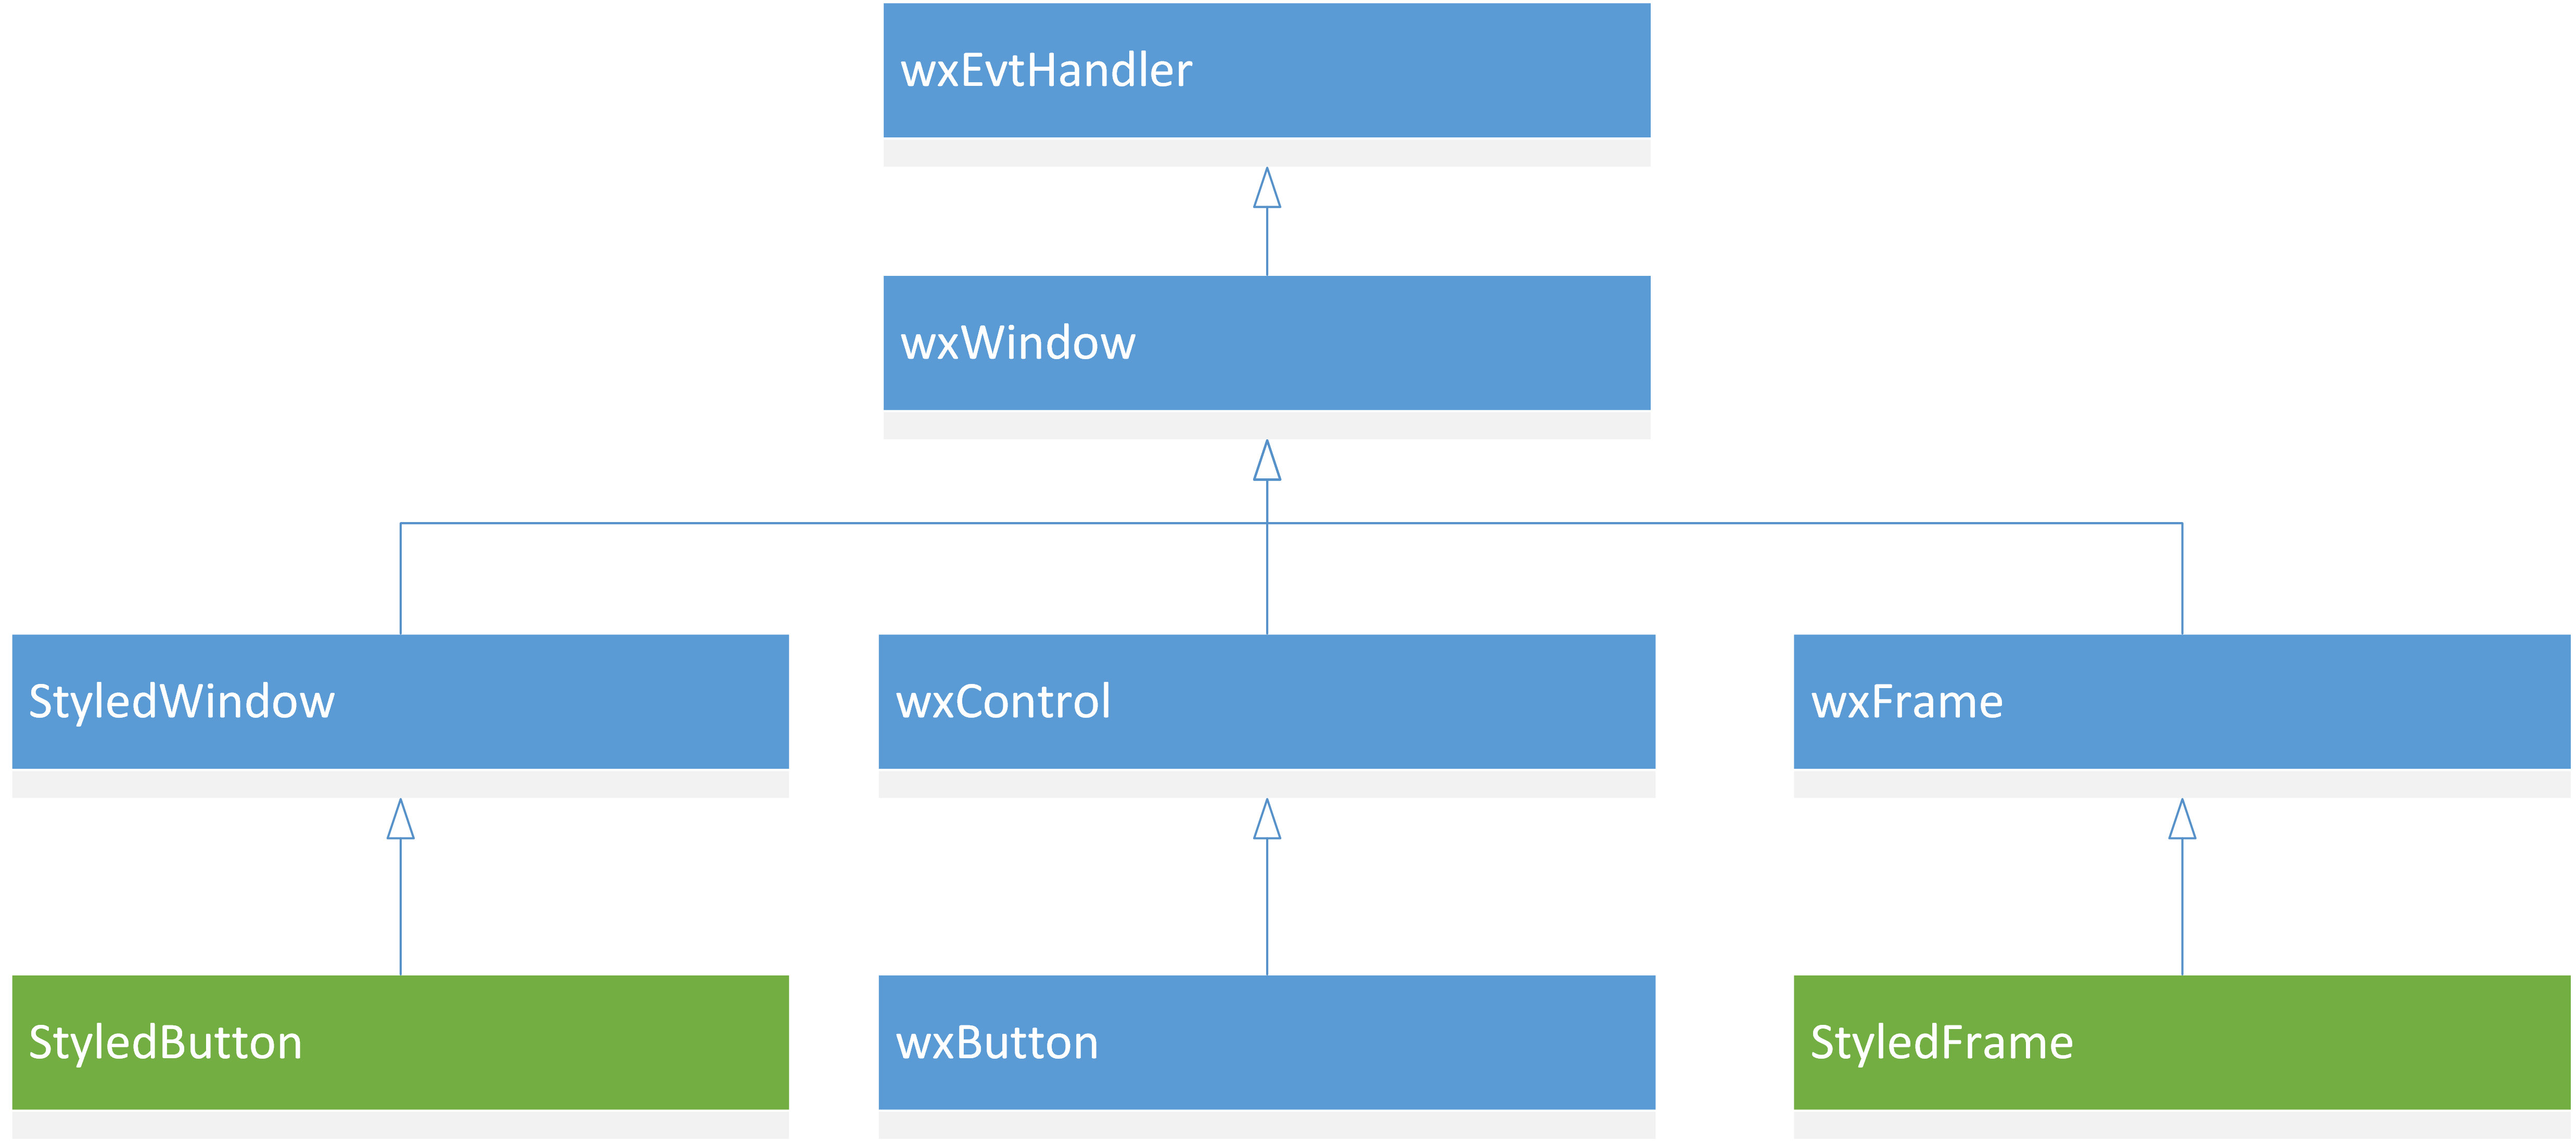
\includegraphics[scale=0.7]{img/ch5_class_system_architecture.png}
    \label{fig:ch5_class_system_architecture}
    \caption{Ierarhia de clase reprezentative pentru obiectele de interfa't'a ale bibliotecii wxStyle}
\end{figure}
\end{center}

Din nefericire mecanismul de procesare al evenimentelor implementat in wxWidgets nu permite legarea mai multor proceduri de procesare aceluia'si eveniment. Acest impediment este tratat 'in interiorul clasei StyledWindow folosind pattern-ul Observer 'in felul urmator:

\medskip

Clasa StyledWindow se conecteaz'a la toate evenimentele de interes pentru obiectele de interfa't'a din libr'aria wxStyle, cum ar fi evenimente de interac'tiune utilizator prin dispozitivul mouse sau tastatur'a, dar 'si evenimente de focus 'si desenare.
Clasa StyledWindow declar'a metode virtuale specializate pentru fiecare eveniment 'si care vor fi apelate 'in cazul intercept'arii evenimentului propriu-zis.
Clasa StyledWindow administreaz'a o list'a de obiecte de tip Listener: MouseListener, KeyboardListener, FocusListener and SizeListener. Aceste interfe'te declar'a metode de procesare a evenimentelor corespunz'atoare fiec'arei categorii. 'In urma apelului de metod'a virtual'a specializat'a pentru eveniment, clasa StyledWindow apeleaz'a metoda specializat'a din interiorul obiectelor de tip Listener care ii sunt ata'sate.

\medskip

[ diagrama UML de clase ]

\medskip

Tot 'in cadrul clasei StyledWindow se afl'a 'si suportul pentru stilizare 'si prezentare customizat'a (custom renderer). Acest lucru se face prin agregarea 'in cadrul clasei a unei instan'te de \emph{Style} 'si a uneia de \emph{StyledRenderer}. At{\ia}t clasele derivate dar 'si utilizatorii acestora pot folosi metode de tip Set 'si Get pentru a schimba instan'tele agregate. Pentru a implementa suportul pentru stilizare, clasa StyledWindow apeleaza medota de prezentare 'si desenare a instan'tei de StyledRenderer 'in cadrul proces'arii evenimentelor de tip Paint.

[ diagrama de comunicare ]

% ==============================================================================
%   Styled Frame
% ==============================================================================

\subsection{StyledFrame}

Obiectul de interfa't'a StyledFrame are rolul de a reprezenta o fereastr'a top-level. Ferestrele sunt compuse din:

\begin{itemize}
\item Cadrul 'si decora'tiunile de cadru care delimiteaz'a suprafa'ta ferestrei 'si permit redimensionarea acesteia.
\item Bara de titlu care con'tine icoana, titlul 'si ac'tiunile minimize, maximize 'si close ale ferestrei.
\item Zona de con'tinut unde sunt agregate obiectele de interfa't'a componente ale fiec'arei ferestre.
\end{itemize}

\begin{center}
\begin{figure}[H]
    \centering
    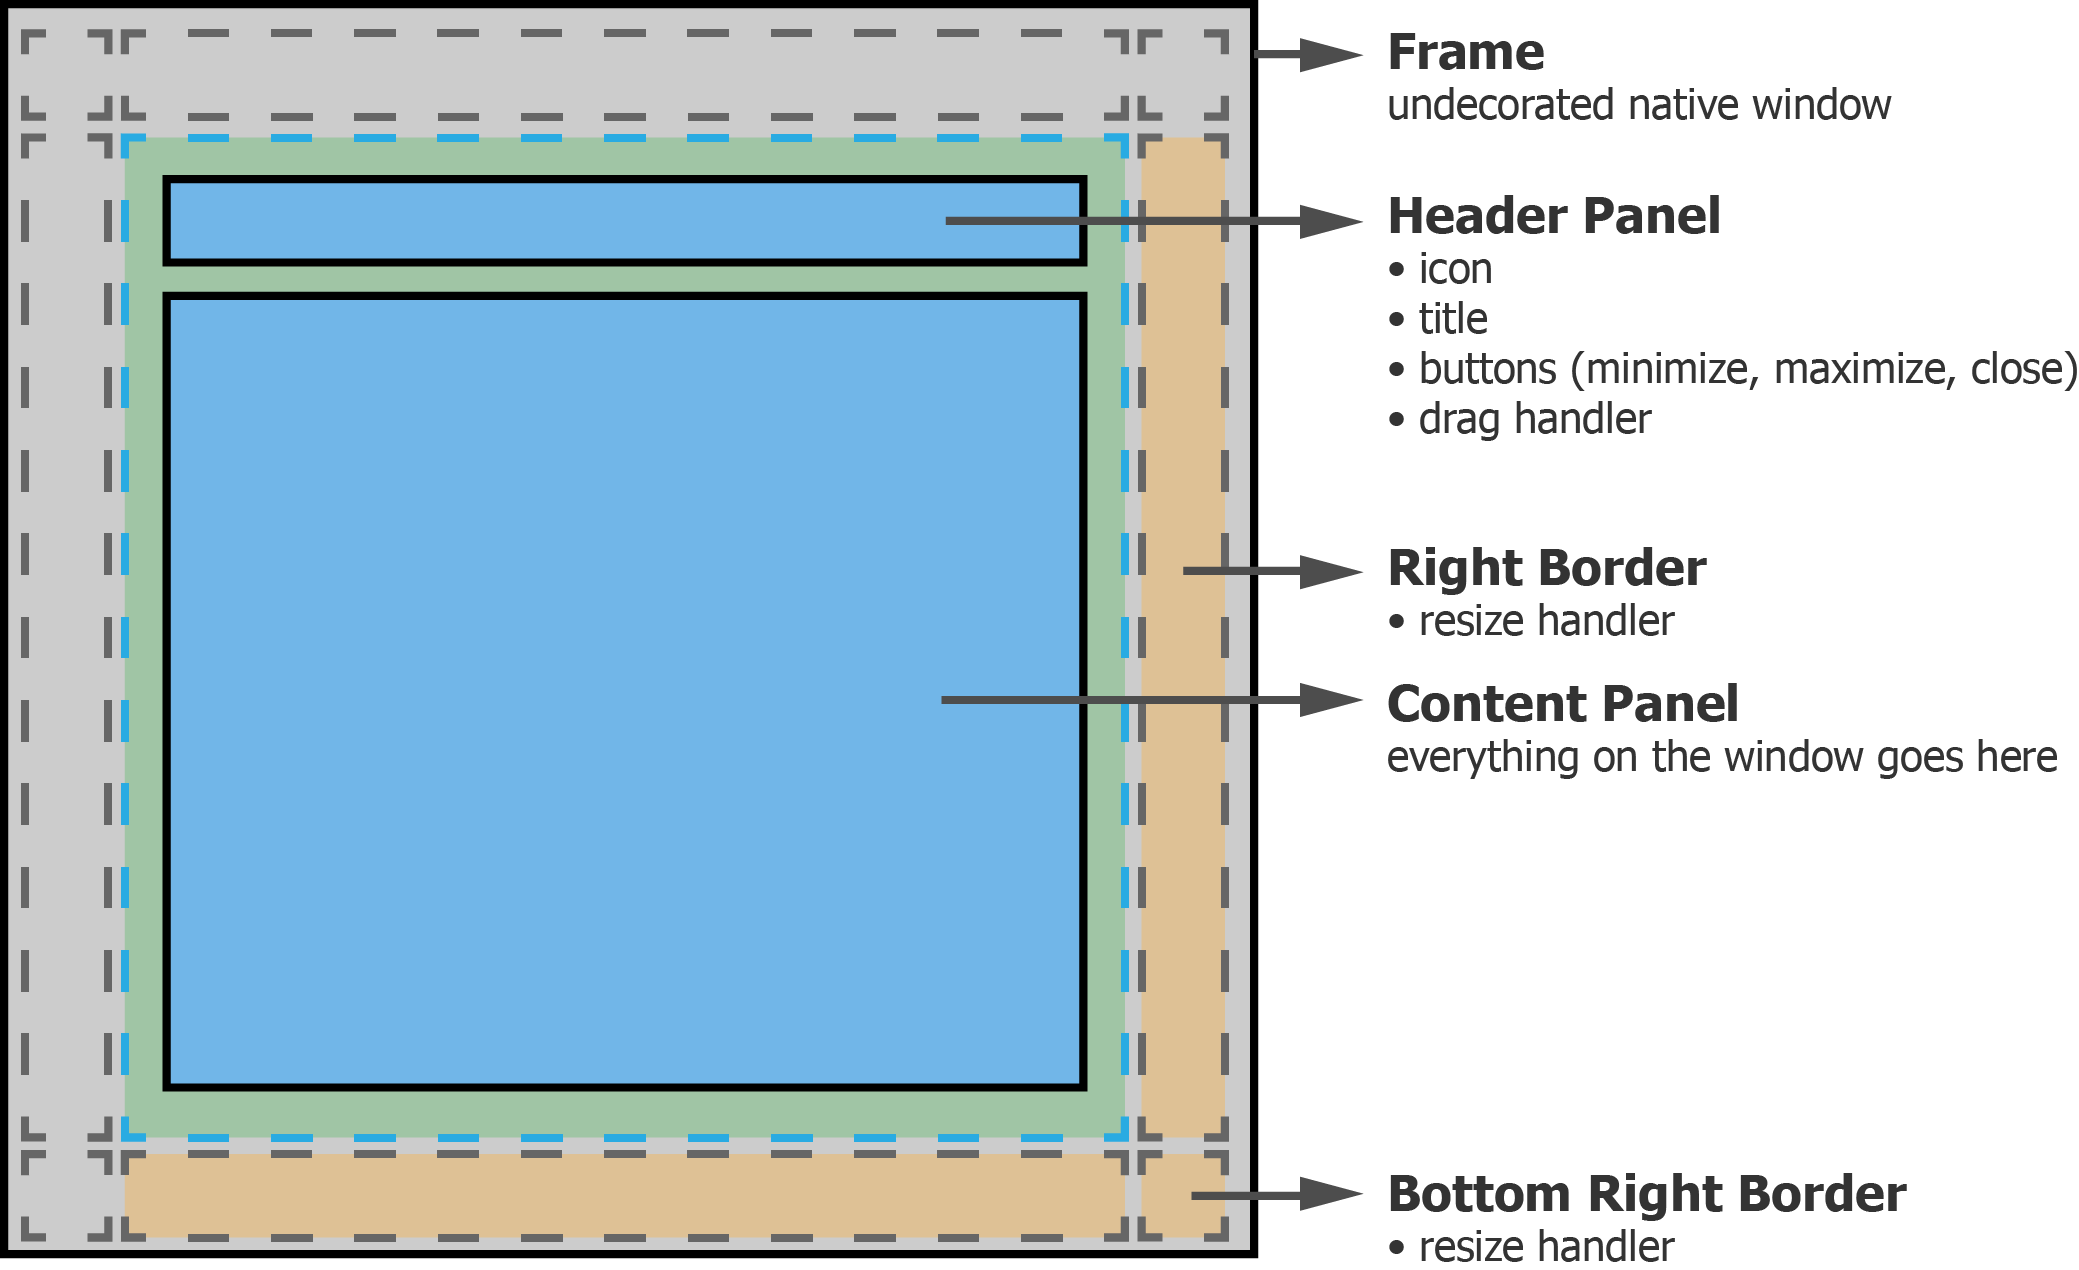
\includegraphics[scale=0.8]{img/ch5_styledframe.png}
    \label{fig:fig_5_2}
    \caption{Structura unei ferestre StyledFrame}
\end{figure}
\end{center}

Obiectul StyledFrame nu face parte din ierarhia de clase ce 'i'si are r'ad'acina 'in clasa StyledWindow deoarece o fereastr'a nu beneficiaz'a de acelea'si tr'as'aturi stilizabile comune celorlalte obiecte de interfa't'a. Aceasta este doar un container pentru ele. Mai mult, in cadrul ierarhiei wxWidgets, ferestrele sunt abstractizate prin clasa wxFrame care este mai specific'a decat wxWindow. Din acest motiv clasa p'arinte a clasei StyledFrame este wxWindow.

\medskip

Totu'si, ferestrele ar trebui s'a permit'a stilizare 'in privin'ta cadrului 'si a b'arii de titlul. Pentru a face acest lucru posibil, StyledFrame construie'ste o fereastr'a nativ'a nedecorat'a, adic'a o fereastr'a care nu con'tine cadru 'si bara de titlul. Pentru a oferii aceea'si func'tionalitate, 'in interiorul ferestrei nedecorate sunt ad'augate componente pentru cadru 'si titlul. 

\medskip

Cadrul este format din 8 panouri speciale distribuite pe marginile ferestrei care pot fi pictate individual pentru a construi orice aspect. La evenimentele de tip Mouse ale acestor panouri se ata'seaz'a componente speciale numite ResizeHandler. Aceste componente transform'a ac'tiunile de tip \emph{drag} ale panourilor de cadru 'in ac'tiuni de resize pentru fereastra p'arinte. 'In acest fel, panourile ce reprezint'a cadrul ferestrei 'indeplinesc 'si func'tionalitate de zone de redimensionare.

\medskip

Zona de titlu este reprezentat'a de o instan't'a a clasei FrameHeader. Aceast'a clas'a are rolul de a encapsula 'si implementa functionalitatea minim'a a unei b'ari de titlu cum ar fi: prezentarea icoanei, prezentarea titlului 'si prezentarea butoanelor de ac'tiune pentru fereastr'a. Mai mult, instan'ta acestei clase din cadru ferestrei poate fi schimbat'a, permi't{\ia}nd utilizatorului s'a construiasc'a ferestre cu b'ari de titlu customizabile 'si stilizabile. La evenimentele de tip Mouse ale acestei clase se ata'seaz'a o component'a de tip DragHandler. Aceast'a component'a are rolul de a interpreta ac'tiunile de tip \emph{drag} executate 'in interiorul zonei de titlu 'in evenimente de repozi'tionare a ferestrei.

\medskip

[ Diagrama UML cu toate clasele participante ]

% ==============================================================================
%   Styled Label
% ==============================================================================

\subsection{StyledLabel}

\begin{center}
\begin{figure}[h]
    \centering
    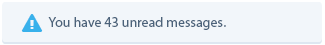
\includegraphics{img/ch5_styledlabel.png}
    \label{fig:fig_5_1}
    \caption{O posibil'a reprezentare a unui obiect de interfa'ta StyledLabel}
\end{figure}
\end{center}

Obiectul de interfa't'a \emph{label} este utilizat pentru prezentarea unui text needitabil. Acesta are de cele mai multe ori rolul de a indica scopul unui alt obiect de interfa't'a, dar poate fi folosit 'si pentru a comunica mesaje / avertismente / erori utilizatorului. Un label con'tine un mesaj text 'si o icoan'a. Mesajul 'si icoana pot fi aliniate in toate cele 9 direc'tii ale dreptunghiului care le con'tine.

[Interfa'ta unui label]

% ==============================================================================
%   Styled Button
% ==============================================================================

\subsection{StyledButton}

Un buton reprezint'a o ac'tiune 'si poate fi activat prin ap'asarea dispozitivului mouse pe suprafa't'a acestuia. 'In timpul ap'as'arii, butonul intr'a 'intr-o stare \emph{armat'a} atunci c{\ia}nd este ap'asat. 'In momentul ridic'arii butonului, acesta declan'seaz'a evenimentul de activare 'si notific'a to'ti observatorii de producerea acestui eveniment. Implementarea butonului presupune procesarea evenimentelor generate de dispozitivul mouse pentru a detecta ap'asarea 'si eliberarea butonului. 

[Interfata unui buton, Interfata unu observator]

% ==============================================================================
%   Styled Checkbox
% ==============================================================================

\subsection{StyledCheckBox}

Obiectul de interfa't'a checkbox reprezint'a o valoarea logic'a. Acesta poate fi activat sau nu, fapt indicat prin bifarea sau cur'a'tarea unei c'asu'te. Obiectele checkbox au ata'sate un mesaj text care indic'a scopul valorii reprezentate. Textul este de cele mai multe ori aliniat la dreapta fa't'a de c'asu'ta indicatoare. Pentru implementarea unui obiect checkbox, trebuie s'a memor'am valoarea pe care o de'tine, 'si sa reac'tion'am la evenimentele dispozitivului mouse de ap'asare 'si eliberare pentru a schimba valoarea obiectului. Unui obiect checkbox i se poate ata'sa un observator care s'a fie notificat 'in momentul schimb'arii valorii obiectului.

[Interfa'ta unui checkbox, interfa't'a unui observator.]

% ==============================================================================
%   Styled TextBox
% ==============================================================================

\subsection{StyledTextBox}

Capitolul de fa'ta are ca subiect implementarea obiectului de interfa't'a StyledTextBox ce permite introducerea 'si editarea de mesaje text. 

\begin{center}
\begin{figure}[h]
    \centering
    
\includegraphics{img/ch5_styledtextbox.png}
    \label{fig:fig_5_1}
    \caption{Editorul de text StyledTextBox}
\end{figure}
\end{center}

\medskip

Acest obiect este reprezentat de o c'asu't'a text 'si un cursor. 'In interiorul c'asu'tei text este prezentat mesajul introdus 'impreuna cu pozi'tia cursorului. De'si textul poate avea o lungime mai mare dec{\ia}t c'asu'ta ce 'il con'tine, caz 'in care va fi prezentat'a doar o parte a textului, cursorul trebuie s'a fie 'intotdeauna 'in interiorul c'asu'tei. Cursorul indica pozi'tia la care noile caractere vor fi introduse in mesajul text. Prin ad'augarea de caractere noi, cursorul i'si schimb'a pozi'tia.

\medskip

Tr'as'aturile 'si functionalitatea pe care un editor de text trebuie s'a le aib'a sunt:

\begin{itemize}
\item Introducerea de text prin ap'asarea tastelor ce reprezint'a caracterele mesajului sau prin alipirea de caractere salvate in \emph{Clipboard}.
\item Navigarea cursorului prin taste (st{\ia}nga, dreapta, home, end, etc.)
\item Navigarea cursorului prin mouse: ap'asarea butonului st{\ia}ng al mouse-ului deasupra textului deja introdus plaseaz'a cursorul 'in cea mai apropiat'a pozitie valid'a relativ la indicatorul mouse-ului.
\item Afi'sarea selectiv'a a textului astfel 'inc{\ia}t cursorul s'a fie 'intotdeauna 'in interiorul c'asu'tei text.
\item Selectarea textului prin taste sau prin mouse astfel 'inc{\ia}t cursorul s'a fie pozi'tionat 'intotdeauna la cap'atul selec'tiei.
\item Editarea textului selectat prin 'stergere sau 'inlocuire.
\item Posibilitatea revoc'arii ac'tiunilor prin func'tionalitate de tip \emph{undo} 'si \emph{redo}.
\end{itemize}

\medskip

Obiectul de interac'tiune implementat de libr'aria wxStyle implementeaz'a toate aceste tr'as'aturi, mai pu'tin posibilitatea anul'arii ac'tiunilor. Interac'tiunea cu utilizatorul se face prin interceptarea 'si interpretarea mesajelor generate de ac'tiunile utilizatorului precum: \emph{MouseMove}, \emph{MouseDown}, \emph{KeyPressed} 'si \emph{KeyChar}. Acestea sunt interceptate 'in super-clasa StyledWindow 'si pot fi procesate prin suprascrierea metodelor virtuale specifice fiec'arui mesaj.

\subsubsection{Introducere Text}

Introducerea textului se face prin inteceptarea mesajelor de tip \emph{KeyChar} care sunt transmise la ap'asarea unei taste ce reprezint'a un caracter vizibil ce nu a fost procesat prin interceptarea unui mesaj de tipul \emph{KeyPressed}.\footnote{http://docs.wxwidgets.org/3.0/classwx\_key\_event.html} Acest mesaj contine caracterul vizibil introdus 'si 'tine cont de starea tastelor \emph{CapsLock} respectiv \emph{Shift} care pot schimba caracterul reprezentat de celelalte taste.

\medskip

Caracterul con'tinut 'in mesaj este introdus 'in textul obiectului de interfa't'a la pozi'tia cursorului. Dac'a exist'a o selec'tie a textului in momentul introducerii caracterului, aceasta va fi inlocuit'a de noul caracter. 'In urma introducerii unui caracter, cursorul i'si schimb'a pozi'tia cu un caracter la dreapta, astfel inc{\ia}t noul caracter s' se afle in st{\ia}nga cursorlui. Dac' noua pozi'tie a cursorului 'il determin'a sa se afle in afara c'asu'tei de text, textul este mutat spre st{\ia}nga sau spre dreapta cu o distan'ta suficient de mare pentru a pozi'tiona cursorul la marginea st{\ia}ng'a respectiv dreapt'a a casu'tei text. Desenarea textului se face folosind un dreptunghi de t'aiere (clipping) care nu las'a textul ce nu se 'incadreaz'a in casu'ta de text, lu{\ia}nd 'in considerare marginile (insets), sa fie desenat.

\medskip

Introducerea textului prin alipire se face prin interceptarea mesajelor de tip \emph{\emph{KeyPressed}} ce descriu ap'asarea tastei \emph{V} 'impreun'a cu modificatorul \emph{Ctrl}.

\subsubsection{Navigare}

Navigarea prin taste se face prin interceptarea acelor mesaje de tip \emph{\emph{KeyPressed}} care au ca surs'a ap'asarea tastelor specifice navig'arii. Astfel, fiecare tasta predefinit'a determina repozi'tionarea cursorului la un nou index. Navigarea prin taste poate determina 'si terminarea selec'tiei printr-un eveniment de navigare ce nu modific'a selec'tia curent'a (ex. tasta \emph{Shift} nu apare ca modificator 'in compozi'tia evenimentului).

\medskip

Navigarea prin mouse se face intercept{\ia}nd acele mesaje de tip \emph{MouseDown} ce nu afecteaz'a starea de focus a obiectului. Prin ap'asarea butonului st{\ia}ng al mouse-ului se parcurge textul deja introdus pentru a g'asi index-ul al c'arui pozi'tie 'in spa'tiul c'asu'tei text este cel mai apropiat de pozi'tia indicatorului.

\subsubsection{Selec'tie}

Selec'tia este reprezentat'a de doi indexi: unul de 'inceput 'si unul de sf{\ia}r'sit. Indexul de 'inceput este 'intotdeauna ini'tializat la pozi'tia cursorului 'in momentul 'inceperii selec'tiei. Indexul de sf{\ia}r'sit este 'intotdeauna acela'si cu indexul cursorului. Modificarea selec'tiei se face 'in mod similar navig'arii normale. Dac'a evenimentul determin'a o schimbare in selec'tia curent'a, indexul de sf{\ia}r'sit al selec'tiei este actualizat la noua pozi'tie a cursorului. Din acest motiv, orice eveniment de navigare poate modifica selec'tia curent'a.

\medskip

'In momentul introducerii de text nou, fie prin alipire, fie prin modul standard, textul descris de selec'tia curent'a este eliminat. 'In acela'si fel, evenimentele de 'stergere ac'tioneaz'a mai 'int{\ia}i asupra selec'tiei curente dac'a exist'a, iar dac'a nu exist'a selec'tie, asupra caracterelor din vecin'atatea cursorului.

\medskip

Selec'tia 'intregului text este posibil'a prin procesarea mesajelor de tip \emph{KeyPressed} ce descriu ap'asarea tastei \emph{A} 'impreun'a cu modificatorul \emph{Ctrl}.

\subsubsection{Prezentare 'si desenare}

Prezentarea este implementat'a 'in cadrul prezentatorului implicit numit StyledTextBoxRenderer, care este privat implementat 'in sursa .cpp ce con'tine 'si implementarea obiectului de interfa'ta. Prezentatorul are rolul de a desena fundalul c'asu'tei text, textul, cursorul 'si selec'tia. Desenarea fundalului se face folosind instruc'tiunile de desenare specificate de stilul obiectului. Desenarea textului se face folosind descrierea de font specificat'a 'in stilul obiectului. Selec'tia 'si cursorul sunt desenate conform propriet'a'tilor SelectionColor 'si CursorWidth ale obiectului de interfa't'a.

\subsubsection{Dezvoltari ulterioare}

Obiectul de interfa't'a StyledTextBox implementeaz'a majoritatea tr'as'aturilor necesare unui editor de text, dar 'in acela'si timp 'ii lipsesc unele tr'as'aturi esen'tiale pentru a putea fi folosit confortabil. Printre aceste tr's'aturi ce lipsesc, amintim c{\ia}teva mai importante:

\begin{itemize}
\item Ac'tiuni de tipul \emph{undo} 'si \emph{undo} a acestui obiect de interfa'ta prin encapsularea ac'tiunilor 'in comenzi structurate 'intr-o stiv'a a istoricului.
\item Posibilitatea ascunderii textului pentru introducerea de informa'tie sensibil'a precum parole.
\item Posibilitatea filtr'arii caracterelor acceptate pentru a construi editoare de numere.
\end{itemize}

% ==============================================================================
%   Infrastructura
% ==============================================================================

\section{Infrastructur'a}

\subsection{Definitiile de stil}

Defini'tiile de stil sunt structuri de date care memoreaz'a asocierea dintre o proprietate a unui obiect de interfa't'a 'si valoarea aceasteia. Pentru a facilita construc'tia de defini'tii par'tiale, vom folosi biblioteca \emph{Boost Optional} care ne permite s'a re'tinem fie o valoare concret'a, fie o valoare goal'a. 'In acest fel putem construi o metod'a care s'a compun'a doua defini'tii de stil verific{\ia}nd care propriet'a'ti sunt setate 'si care nu.

[class diagram]

\subsection{Instructiunile de desenare}

Instruc'tiunile de desenare au rolul de a encapsula o metod'a de desenare 'si parametrii acesteia. Instruc'tiunile de desenare sunt simple clase care agreg'a valorile parametrilor instruc'tiunii 'si implementeaz'a o metod'a de desenare 'in cadrul c'areia se apeleaza instruc'tiunea propriu-zis'a.

[class diagram]

\subsection{Dimensiuni Uniforme}



\subsection{Procesoare de mi'scare 'si redimensionare a ferestrelor}

Procesoarele de mi'scare 'si redimensionare sunt folosite 'in implementarea ferestrelor pentru a procesa evenimentele produse de dispozitivul mouse 'si de a le '

\subsection{Mecanismul de identificare al tipurilor de obiecte (RTTI)}

\subsection{Cititorul de fi'siere de stil}

% ==============================================================================
%   Prezentare si desenare
% ==============================================================================

\section{Prezentarea 'si desenare obiectelor de interfa't'a}

Pentru a prezenta un obiect de interfa't'a, utiliz'am primitivele de desenare oferite de wxWidgets. Acestea sunt \emph{wxDC}\footnote{http://docs.wxwidgets.org/3.0/classwx\_d\_c.html} care reprezint'a un dispozitiv ce suport'a desenare 'si \emph{wxGraphicsContext}, o clas'a ce permite desenarea de obiecte grafice primitive pe suprafa'ta unui dispozitiv. 

\subsection{Dispozitive de desenare wxDC}

Un dispozitiv poate fi un fi'sier raster, un fi'sier vectorial, o imprimant'a sau suprafa'ta unei ferestre. Mai mult dec{\ia}t reprezentarea unei destina'tii pentru desenare, obiectele de tipul wxDC ofer'a 'si metode pentru desenarea efectiv'a. Pentru suprafa'ta unei ferestre, wxWidgets pune la dispozi'tie mai multe tipuri de DC-uri, precum \emph{wxClientDC}, \emph{wxWindowDC}, \emph{wxPaintDC}, \emph{wxBufferedPaintDC}, \emph{wxAutoBufferedPaintDC}.

\begin{itemize}
\item \textbf{wxWindowDC} ofer'a posibilitatea desen'arii pe 'intreaga suprafa't'a a unei ferestre, inclusiv marginile 'si decora'tiunile. Acest lucru este suportat doar pe sistemul de operare Windows.
\item \textbf{wxClientDC} ofer'a posibilitatea desen'arii 'in interiorul unei ferestre, 'in zona denumit'a zona client.
\item \textbf{wxPaintDC} este utilizat pentru a desena pe suprafa'ta client a unei ferestre 'in cadrul unei metode de procesare a evenimentului de desenare. Acest obiect are 'si rolul de a construi regiunea de clipping a ferestrei. wxWidgets necesit'a construirea unui astfel de obiect 'in interiorul metodei de procesare a evenimentelor de desenare, indiferent dac'a obiectul este folosit sau nu.
\item \textbf{wxBufferedPaintDC} este un device context de tipul \emph{buffered}, adic'a are suport pentru evitarea artefactelor de tipul \emph{flicker}. Este de asemenea un device context de tipul \emph{Paint}, adic'a poate fi folosit pentru a procesa evenimentele de desenare.
\item \textbf{wxAutoBufferedPaintDC} prezint'a o 'imbun'at'a'tire fa't'a de \emph{wxBufferedPaintDC} deoarece nu implementeaz'a procesul de double-buffering pe platformele care suport'a nativ acest lucru. Pentru a utiliza acest device context, este necesar specificarea stilului wxBG\_STYLE\_PAINT care previne procesul separat de desenare al fundalului.
\end{itemize}

'In urma test'arii fiec'arui tip de device context, cel mai potrivit s-a demonstrat a fi \emph{wxAutoBufferedPaintDC}. Acest lucru se datoreaz'a faptului ca elimina artefactele de tipul \emph{flicker} care sunt evidente 'si deranjante, 'in special 'in momentele 'in care un obiect de interfa't'a 'i'si schimb'a 'inf'a'ti'sarea datorit'a unei schimb'ari de stare. De asemenea, acest obiect este mai performant dec{\ia}t fratele s'au \emph{wxBufferedPaintDC}. Din nefericire, \emph{wxAutoBufferedPaintDC} presupune desenarea pe o suprafa't'a (imagine) intermediar'a, care este ini'tializat'a cu o culoare uniform'a neagr'a. Acest lucru previne posibilitatea de transparen't'a a obiectelor de interfa't'a. 

Lipsa de transparen'ta presupune imposibilitatea de desenare a unor obiecte de interfa't'a cu alte forme dec{\ia}t dreptunghiul care le delimiteaz'a. Un pas 'in rezolvarea acestei probleme a fost implementarea unui mecanism de g'asire a culorii de fundal 'in func'tie de ierarhia p'arin'tilor 'si proprietatea de transparen't'a a acestora. Algoritmul recursiv este urm'atorul:

\begin{enumerate}
\item Dac'a obiectul este opac, utilizeaz'a culoarea de fundal a obiectului.
\item Dac'a obiectul este transparent:
	\begin{enumerate}
	\item Dac'a are p'arinte, utilizeaz'a culoarea de fundal a parintelui.
	\item Dac'a nu are p'arinte, itlizeaz'a o culoare predefinit'a (negru).
	\end{enumerate}
\end{enumerate}

Acest algoritm nu func'tioneaz'a dac'a vreunul dintre p'arin'ti utilizeaz'a unul din procesele de stilizare 'si prezentare puse la dispozi'tie de biblioteca wxStyle. 'In schimb, este util pentru cazul simplu 'in care obiectele de interfa't'a sunt 'incadrate 'intr-o fereastr'a cu un fundal umplut cu o culoare uniform'a.

\subsection{Mecanismul de desenare wxGraphicsContext}

Pentru a acomoda evolu'tia API-urilor pentru desenare grafic'a, wxWidgets a introdus un nou mecanism de desenare prin obiecte de tipul \emph{wxGraphicsContext}. Aceste obiecte sunt construite printr-un \emph{wxRenderer} care reprezint'a unul din API-urile grafice abstractizate de wxWidgets. Printre aceste API-uri, pe platforma Windows sunt disponibile \emph{Cairo}, \emph{GDI+} 'si, mai nou, \emph{Direct2D}. Obiectele de tipul \emph{wxGraphicsContext} sunt ata'sate unui dispozitiv la momentul construc'tiei.

\medskip

Diferit fa't'a de API-ul pentru desenare oferit de obiectele \emph{wxDC}, \emph{wxGraphicsContext} lucreaz'a cu obiecte speciale numite \emph{wxGraphicsObjects} care descriu pensule, peni'te, traiectorii 'si matrici de transfomare. Aceste obiecte encapsuleaz'a 'si abstractizeaz'a obiectele native ale API-ului grafic, 'si fac leg'atura cu obiectele specializate wxWidgets precum \emph{wxPen}, \emph{wxBrush}, etc.

\medskip

Prezentatorii din biblioteca wxStyle folosesc obiecte de tipul wxGraphicsContext pentru a executa instruc'tiunile de desenare. Un exemplu de cod care ini'tializeaz'a un context de desenare pentru a fi folosit in interiorul unei metode de prezentare este prezent in figura \ref{fig0510}. Pentru a asigura dealocarea corect'a 'si distrugerea obiectului de tipul \emph{wxGraphicsContext*}, utiliz'am un pointer inteligent din libr'aria standard C++.

\begin{figure}[H]
\begin{lstlisting}[language=C++]
// g is a pointer to a wxGraphicsContext which is 
// automatically destroyed at the end of the method
wxAutoBufferedPaintDC dc(label);
auto g = unique_ptr<wxGraphicsContext>(wxGraphicsContext::Create(dc)).get();
\end{lstlisting}
\caption{Exemplu de ini'tializare al unui wxGraphicsContext}
\label{fig0510}
\end{figure}